\chapter{RADAR Basics}\label{chapter_radar_basics}
This chapter covers some RADAR basics, including the RADAR range equation, propagation factors, and bistatic configurations.

\section{RADAR Range Equation} 
The RADAR range equation provides a deterministic method to calculate received signal levels and is the workhorse for analyzing RADAR system performance. This equation is the first step towards building a statistical model, as it captures the underlying physics.

\subsection{Monostatic Case}
The RADAR range equation is derived by assuming spherically propagating waves and computing the propagated power at 4 incremental points between the transmitter and target as shown in Figure \ref{intro_fig:1}. These points are the projected power ($P_1$), the power received at the target ($P_2$), the power reflected by the target ($P_3$), and the power at the receiver antenna ($P_4$). The received power ($P_r$) is then the product of $P_4$ and the effective area of the receiver antenna.

\begin{figure}[H]
  \begin{center}
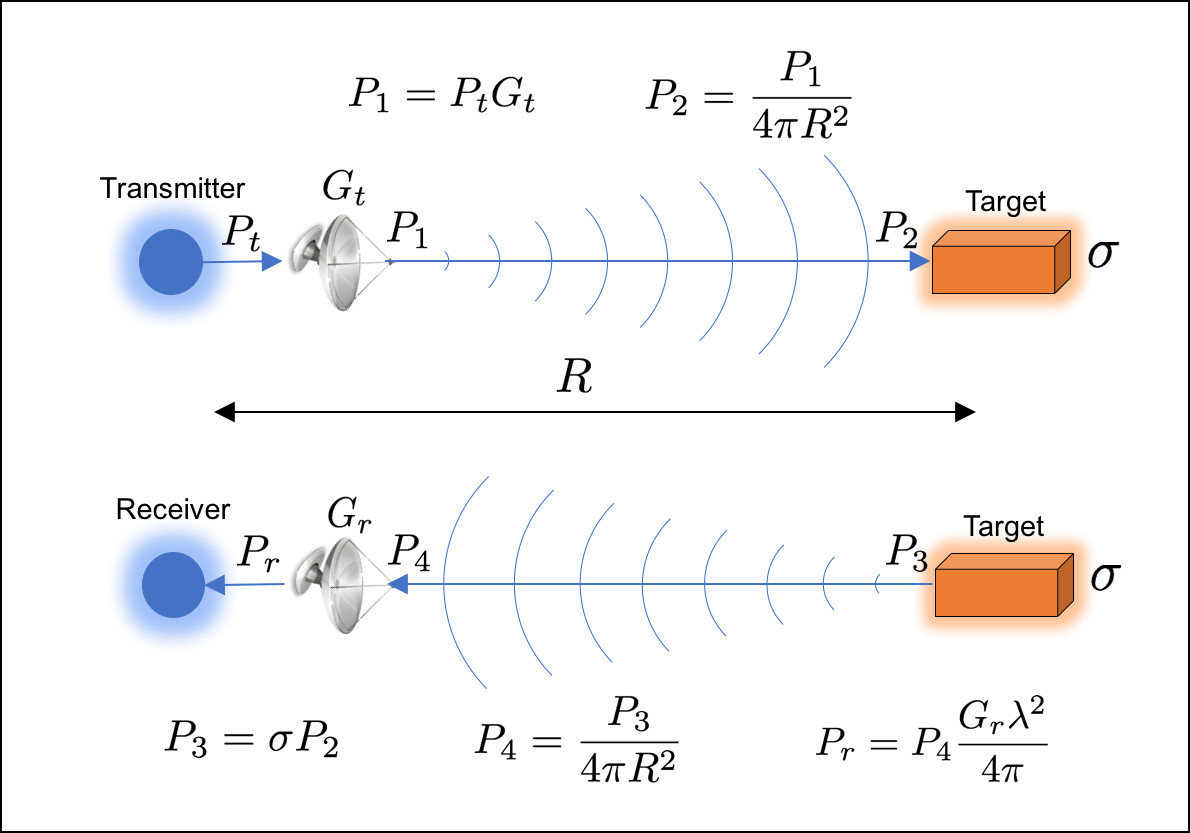
\includegraphics[width=4in]{../media/multistatic/radar_range_equation.png}
  \end{center}
  \renewcommand{\baselinestretch}{1} \small\normalsize
  \begin{quote}
    \caption[RADAR Range Equation Derivation]{RADAR Range Equation Derivation \label{intro_fig:1}}
  \end{quote}
\end{figure}
\renewcommand{\baselinestretch}{2} \small\normalsize

With spherical waves, the power is spread out over a sphere of radius equal to the slant range, $R$, which gives a scaling factor of $\left( 4\pi R^2 \right)^{-1}$ for propagation. The total projected power, $P_1$, is the transmitted power, $P_t$, multiplied by the antenna gain, $G_t$. The RCS, $\sigma$, defines the amount of power reflected, and the effective area of the antenna is $G_t\lambda^2(4\pi)^{-1}$.

In the monostatic case, $G_t = G_r$ and the RADAR range equation is then \cite{skolnik_handbook}.
  \begin{equation}
  \label{intro_eq:1}
 P_r = \frac{P_tG_t^2\sigma\lambda^2}{\left(4\pi\right)^3R^4}
  \end{equation}
In this equation, the antenna gain, $G_t$ is a function of the angle between the antenna boresight and the target. Randomness enters this version of the RADAR range equation through the target RCS as there is otherwise no term to account for environmental fluctuations.

In the atmosphere, propagation is a linear operation. Therefore we can leverage superposition to compute the RADAR range equation for each path or scatterer and sum the results.

We can divide Equation \ref{intro_eq:1} by the noise power to represent the RADAR range equation in terms of signal to noise ratio (SNR) \cite{skolnik_handbook}.
\begin{equation}
    \label{intro_eq:2}
\text{SNR} = \frac{P_r}{P_n} = \frac{P_tG_t^2\sigma\lambda^2}{\left(4\pi\right)^3 R^4k_BTBF_n}
\end{equation}
In this equation, $k_B$ is the Boltzmann constant, $B$ is the receiver bandwidth, $T$ is the receiver temperature and $F_n$ is the receiver noise figure. Nominally, $B$ is taken to be the inverse of the pulse width to accomodate matched filter processing and $T$ is taken to be $300$ K.

\subsection{Bistatic Case}
In the bistatic case, we need to consider each path separately as the ranges, antenna gains, and RCS are all likely different. The standard bistatic RADAR range equation is shown in Equation \ref{intro_eq:3}.
  \begin{equation}
  \label{intro_eq:3}
 P_r = \frac{P_tG_tG_r\sigma_B\lambda^2}{\left(4\pi\right)^3R_1^2R_2^2}
  \end{equation}
In this equation, $G_t$ is the antenna gain for the transmitter, $G_r$ is the antenna gain for the receiver, $\sigma_B$ is the bistatic RCS, $R_1$ is the slant range along the first path (transmitter to target), and $R_2$ is the slant range along the second path (target to receiver). Again, the antenna gains, $G_t$ and $G_r$ are functions of the angle between the antenna boresight and the target.

The bistatic RADAR range equation in terms of SNR is shown in Equation \ref{intro_eq:4}.
\begin{equation}
    \label{intro_eq:4}
\text{SNR} = \frac{P_tG_tG_r\sigma_B\lambda^2}{\left(4\pi\right)^3 R_1^2R_2^2k_BTBF_n}
\end{equation}

\subsection{Propagation Factors}
The use of a propagation factor, $F_p$, allows us to include atmospheric effects in the RADAR range equation. These effects can include absorption from atmospheric gases and weather such as rain or snow as well as rollups for the effects of multipath reflections, diffraction from the surface, and clipping by the horizon. The propagation factor is typically implemented as a multiplier to the RADAR range equation and provides another mechanism to introduce randomness. Because they encompasses a wide variety of environment conditions, propagation factors are generally complicated to compute. 

The bistatic RADAR range equation with a propagation factor included is given in Equation \ref{intro_eq:4a}.
  \begin{equation}
  \label{intro_eq:4a}
 P_r = \frac{P_tG_tG_r\sigma_B\lambda^2}{\left(4\pi\right)^3R_1^2R_2^2}F_p
  \end{equation}
  
To visualize the propagation factors, Figure \ref{intro_fig:1a} shows the propagation factors for standard atmosphere and Figure \ref{intro_fig:1b} shows the propagation factors with a 20 m duct. With standard atmosphere, we can see the impact of the horizon as well as the periodic multipath peaks and nulls. With a 20 m duct, the atmosphere acts as a waveguide (described in detail in Chapter \ref{chapter_env}) so that propagation can extend past the horizon.
  \begin{figure}[H]
  \begin{center}
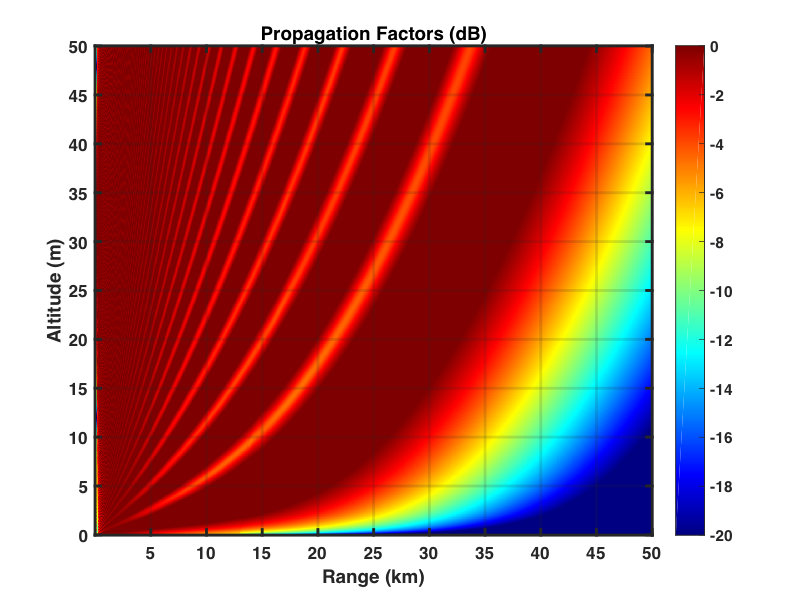
\includegraphics[width=4in]{../media/multistatic/std_atmos_pf.png}
  \end{center}
  \renewcommand{\baselinestretch}{1} \small\normalsize
  \begin{quote}
    \caption[Propagation Factors for Standard Atmosphere]{Propagation Factors for Standard Atmosphere \label{intro_fig:1a}}
  \end{quote}
\end{figure}
\renewcommand{\baselinestretch}{2} \small\normalsize

\begin{figure}[H]
  \begin{center}
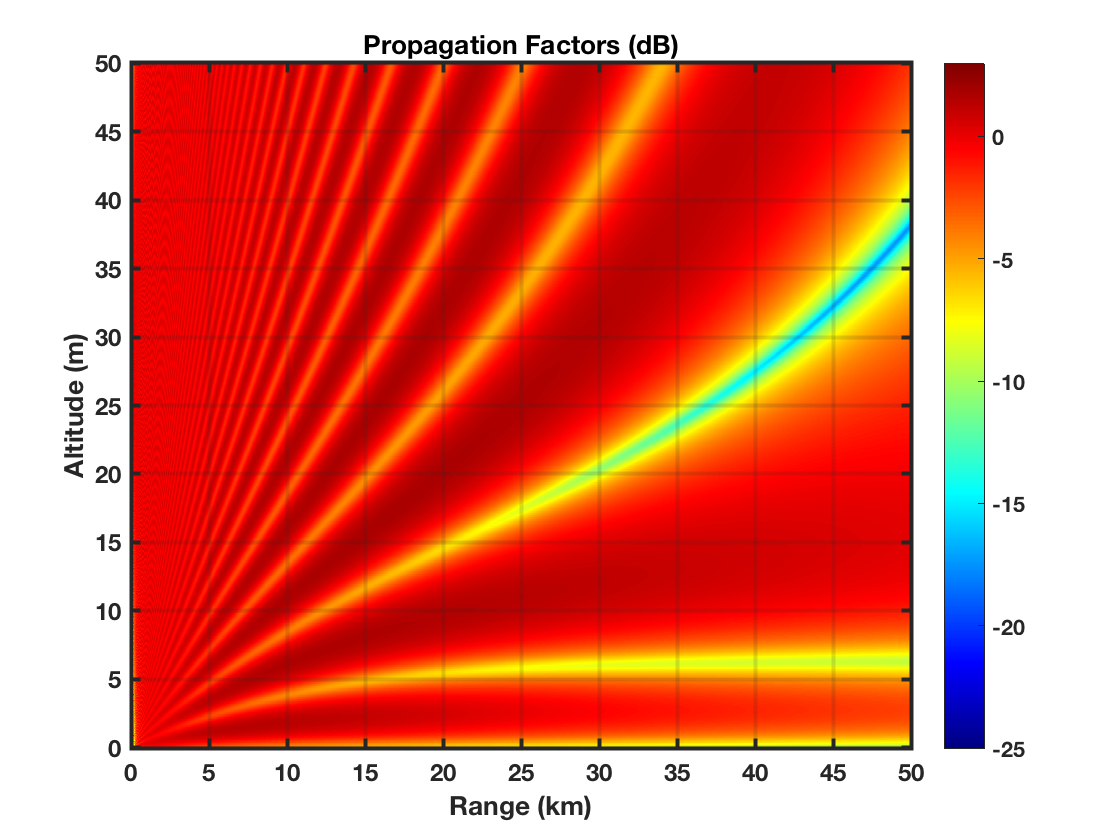
\includegraphics[width=4in]{../media/multistatic/20m_duct_pf.png}
  \end{center}
  \renewcommand{\baselinestretch}{1} \small\normalsize
  \begin{quote}
    \caption[Propagation Factors for a 20 m Duct]{Propagation Factors for a 20 m Duct \label{intro_fig:1b}}
  \end{quote}
\end{figure}
\renewcommand{\baselinestretch}{2} \small\normalsize

\section{Beam Width}
The beam width of an antenna is defined as the angle between the half power points in the antenna pattern. We will use a sinc antenna pattern to demonstrate this concept.

\subsection{One Way Beam Width}
The one way antenna beam width, $\theta$, is simply the beam width of the forward propagating beam. The electric field amplitude in the far field of a sinc antenna pattern is given by Equation \ref{rb_eq:1} and shown in Figure \ref{rb_fig:4}.

\begin{equation}
\label{rb_eq:1}
E(\theta) = \frac{\sin\left(\frac{\pi D}{\lambda}\sin(\theta) \right)}{\frac{\pi D}{\lambda}\sin(\theta)}
\end{equation}

\begin{figure}[H]
  \begin{center}
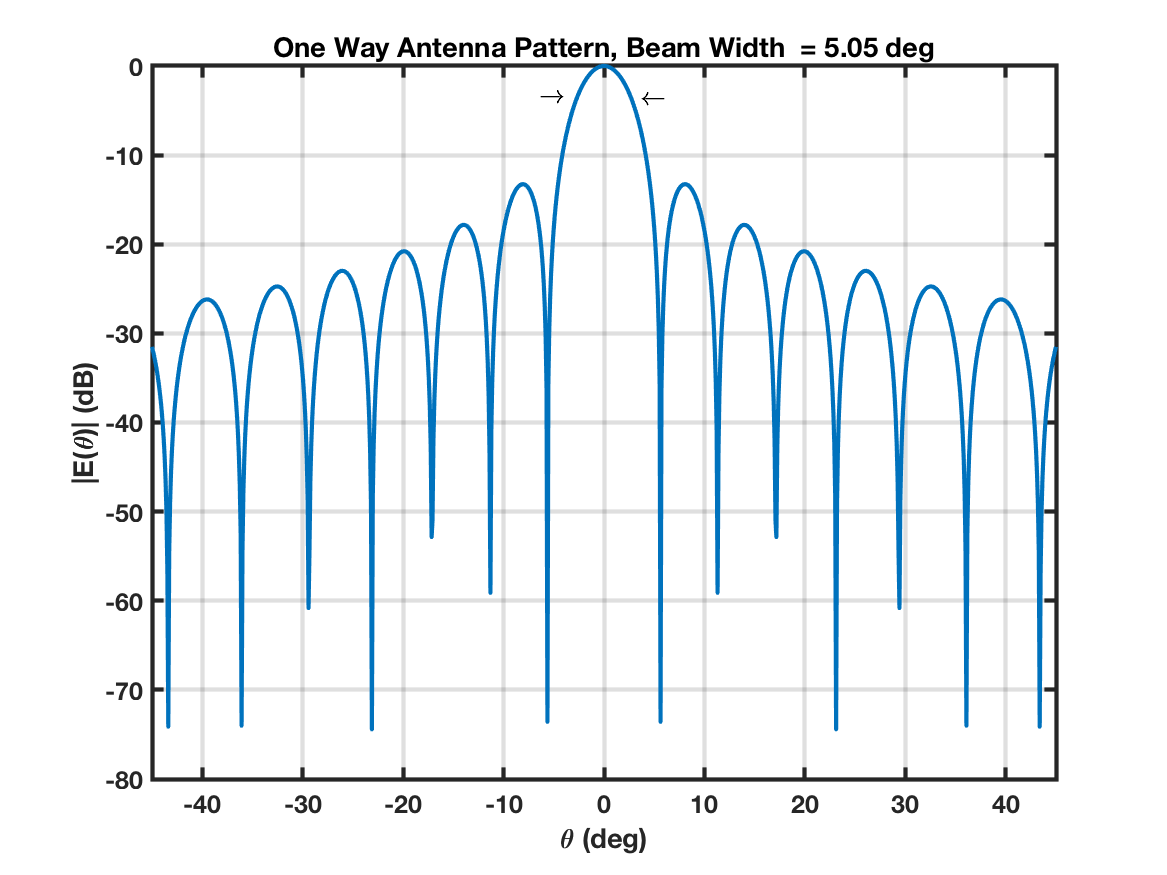
\includegraphics[width=4in]{../media/multistatic/sinc_antenna_pattern_one_way.png}
  \end{center}
  \renewcommand{\baselinestretch}{1} \small\normalsize
  \begin{quote}
    \caption[One Way Antenna Pattern]{One Way Antenna Pattern\label{rb_fig:4}}
  \end{quote}
\end{figure}
\renewcommand{\baselinestretch}{2} \small\normalsize

\subsection{Two Way Beam Width}
The two way antenna beam width, $\theta_2$, is the beam width of the beam propagating in both directions. For the monostatic case, we can compute this as the one way beam width of the square of the antenna pattern. For the sinc pattern, the two way pattern is shown in Figure \ref{rb_fig:5}. In most cases, $\theta_2 \approx \theta/\sqrt{2}$.

\begin{figure}[H]
  \begin{center}
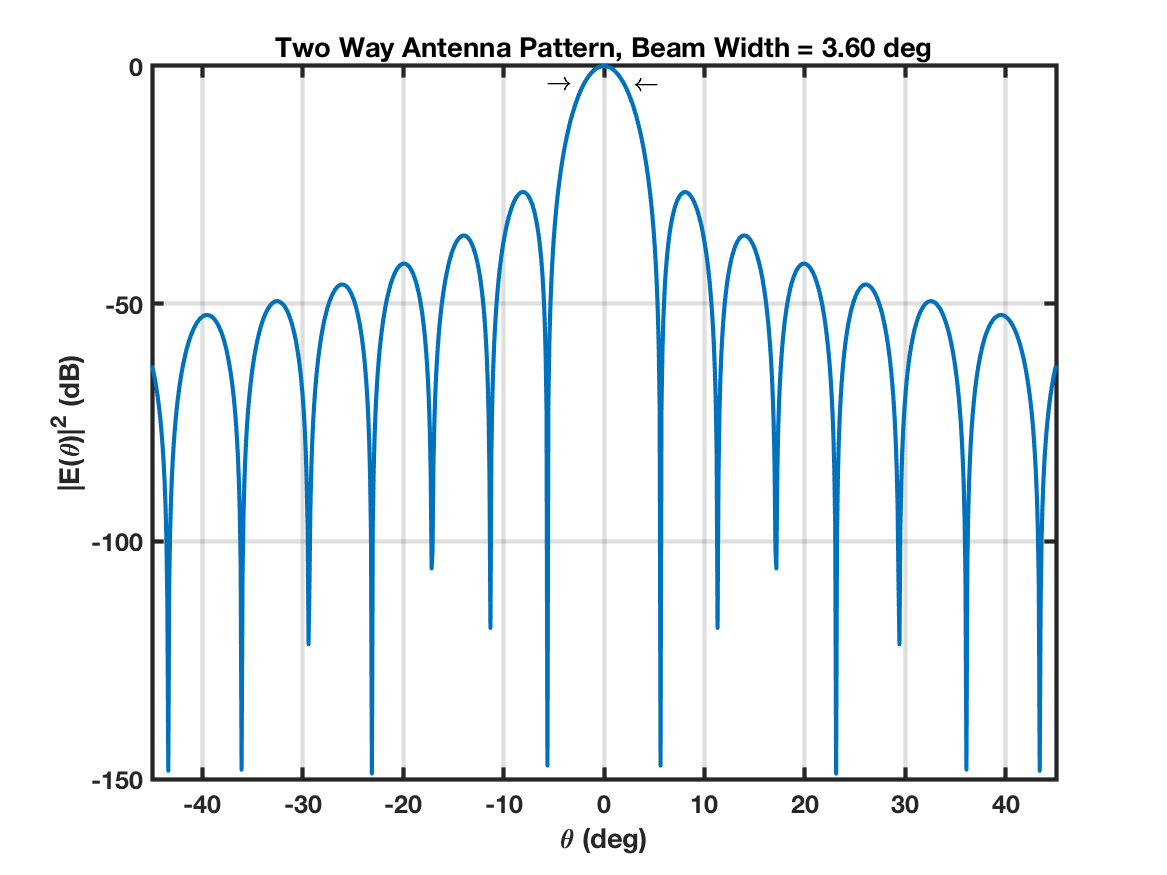
\includegraphics[width=4in]{../media/multistatic/sinc_antenna_pattern_two_way.png}
  \end{center}
  \renewcommand{\baselinestretch}{1} \small\normalsize
  \begin{quote}
    \caption[Two Way Antenna Pattern]{Two Way Antenna Pattern\label{rb_fig:5}}
  \end{quote}
\end{figure}
\renewcommand{\baselinestretch}{2} \small\normalsize
The two way beam width is really only valid for monostatic configurations that assume the forward and backward propagating beams lie directly on top of one another. In a bistatic configuration, the beams overlap differently and need to be explicitly evaluated.

\section{Bistatic Configurations}
Because the transmitter and receiver are not colocated in a bistatic configuration, the geometry now becomes ellipsoidal as shown in Figure \ref{intro_fig:2}. Here, $R_1$ is the slant range from the transmitter to the target, $R_2$ is the slant range from the target to the receiver, $\theta_t$ is the one way beam width of the transmitter and $\theta_r$ is the one way beam width of the receiver. The bistatic angle, $\beta$, is the angle between the transmitter and receiver in the plane containing the transmitter, receiver, and target. 
\begin{figure}[H]
  \begin{center}
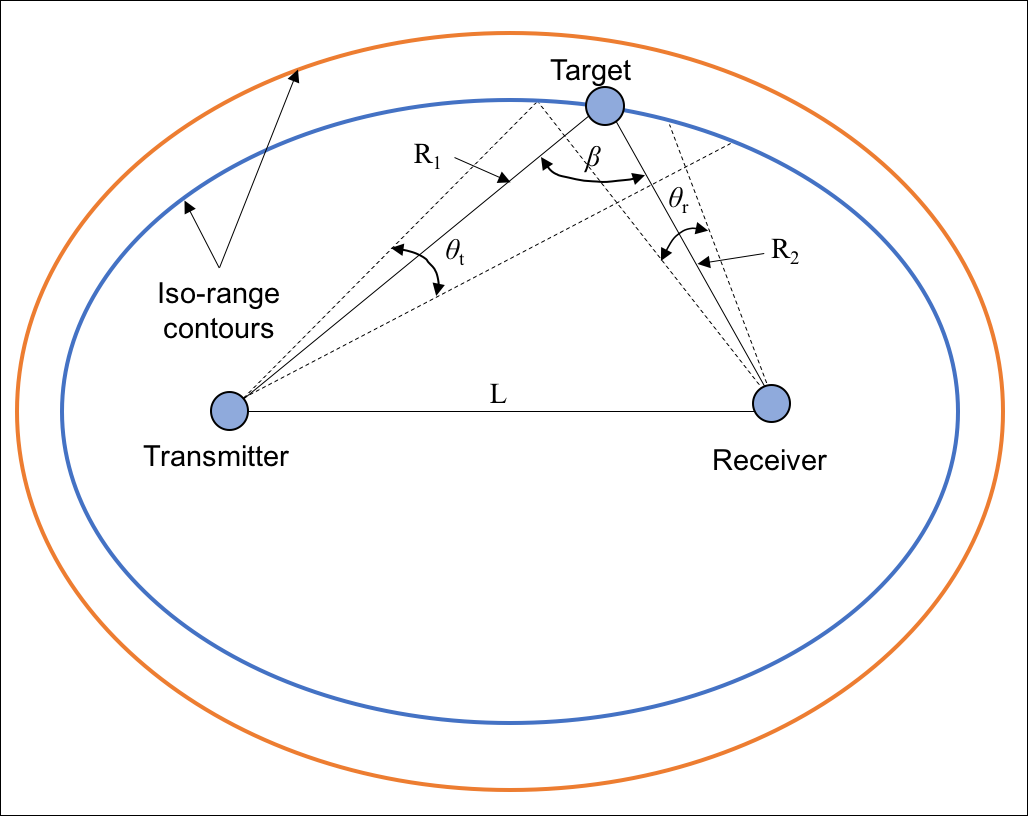
\includegraphics[width=4in]{../media/multistatic/Isorange_contours.png}
  \end{center}
  \renewcommand{\baselinestretch}{1} \small\normalsize
  \begin{quote}
    \caption[Isorange Contours for Bistatic Configuration]{Isorange Contours for Bistatic Configuration \label{intro_fig:2}}
  \end{quote}
\end{figure}
\renewcommand{\baselinestretch}{2} \small\normalsize
The isorange contours are defined as the curves where the total path length, $R_1 + R_2$, is constant . These contours form ellipses with the transmitter and receiver at the foci as shown in the blue and orange curves in Figure \ref{intro_fig:2}. For the monostatic case, the isorange contours are simply circles and the geometry is simplified as everything is symmetric. In the bistatic case, however, the beam width is not symmetric along the isorange contours, which results in skewing the impact of clutter.

It is often convenient to look at things in terms of SNR. In a bistatic configuration, the loci of constant SNR are known as the ovals of Cassini \cite{willis_bistatic} and an example is shown in Figure \ref{intro_fig:3}.
\begin{figure}[H]
  \begin{center}
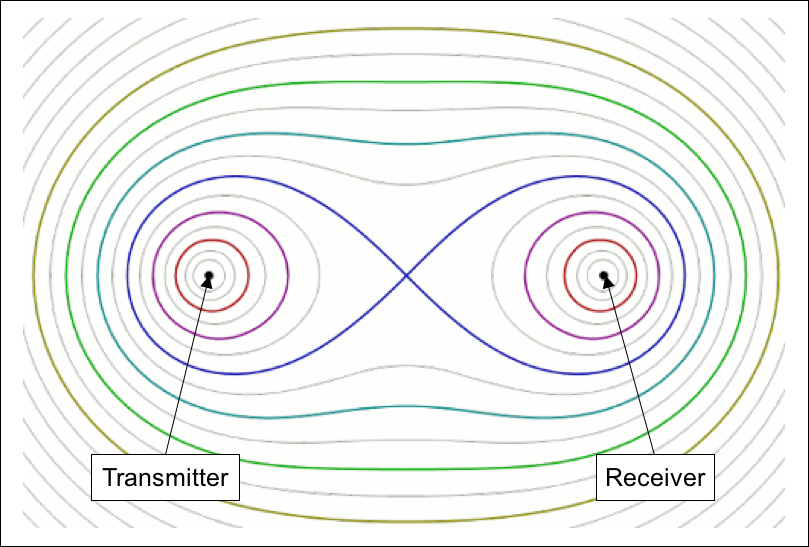
\includegraphics[width=4in]{../media/multistatic/ovals_of_cassini.png}
  \end{center}
  \renewcommand{\baselinestretch}{1} \small\normalsize
  \begin{quote}
    \caption[Ovals of Cassini]{Ovals of Cassini\label{intro_fig:3}}
  \end{quote}
\end{figure}
\renewcommand{\baselinestretch}{2} \small\normalsize
The ovals of Cassini are a simplification that assumes the target RCS and propagation factors are invariant with respect to angle and range. This is rarely the case, but the ovals of Cassini are useful to quickly represent system constraints.

For large SNR, the ovals of Cassini collapse around the transmitter and receiver and define the transmitter centered and receiver centered regions. The cosite region is defined as when the ovals of Cassini surround both the transmitter and receiver \cite {willis_bistatic}.